\documentclass{article}
\usepackage{graphicx, tikz-cd, float, titlepic, booktabs} % Required for inserting images
\usepackage{pgfplots}
\pgfplotsset{compat=1.15}
\usepackage{mathrsfs}
\usetikzlibrary{arrows}
\usepackage{amsmath, amssymb, amsthm, amsfonts, siunitx, physics, gensymb}
\AtBeginDocument{\RenewCommandCopy\qty\SI}
\usepackage[version=4]{mhchem}
\usepackage[most,many,breakable]{tcolorbox}
\usepackage{xcolor, fancyhdr, varwidth}
\usepackage[Glenn]{fncychap}
%Options: Sonny, Lenny, Glenn, Conny, Rejne, Bjarne, Bjornstrup
\usepackage{hyperref, cleveref}
\usepackage{icomma, enumitem} %comma as decimal and continue enumerate with [resume]
\usepackage[danish]{babel}
%%%%%%%%%%%%%%%%%%%%%%%%%%%%%%
% SELF MADE COLORS
%%%%%%%%%%%%%%%%%%%%%%%%%%%%%%
\definecolor{myg}{RGB}{56, 140, 70}
\definecolor{myb}{RGB}{45, 111, 177}
\definecolor{myr}{RGB}{199, 68, 64}
\definecolor{mytheorembg}{HTML}{F2F2F9}
\definecolor{mytheoremfr}{HTML}{00007B}
\definecolor{mylenmabg}{HTML}{FFFAF8}
\definecolor{mylenmafr}{HTML}{983b0f}
\definecolor{mypropbg}{HTML}{f2fbfc}
\definecolor{mypropfr}{HTML}{191971}
\definecolor{myexamplebg}{HTML}{F2FBF8}
\definecolor{myexamplefr}{HTML}{88D6D1}
\definecolor{myexampleti}{HTML}{2A7F7F}
\definecolor{mydefinitbg}{HTML}{E5E5FF}
\definecolor{mydefinitfr}{HTML}{3F3FA3}
\definecolor{notesgreen}{RGB}{0,162,0}
\definecolor{myp}{RGB}{197, 92, 212}
\definecolor{mygr}{HTML}{2C3338}
\definecolor{myred}{RGB}{127,0,0}
\definecolor{myyellow}{RGB}{169,121,69}
\definecolor{myexercisebg}{HTML}{F2FBF8}
\definecolor{myexercisefg}{HTML}{88D6D1}
%%%%%%%%%%%%%%%%%%%%%%%%%%%%%%%%%%%%%%%%%%%%%%%%%%%%%%%%%%%%%%%%%%%%%%
% Box environments for theorems and problems
%%%%%%%%%%%%%%%%%%%%%%%%%%%%%%%%%%%%%%%%%%%%%%%%%%%%%%%%%%%%%%%%%%%%%
\setlength{\parindent}{1cm}
%================================
% Question BOX
%================================
\makeatletter
\newtcbtheorem{question}{Opgave}{enhanced,
	breakable,
	colback=white,
	colframe=myb!80!black,
	attach boxed title to top left={yshift*=-\tcboxedtitleheight},
	fonttitle=\bfseries,
	title={#2},
	boxed title size=title,
	boxed title style={%
			sharp corners,
			rounded corners=northwest,
			colback=tcbcolframe,
			boxrule=0pt,
		},
	underlay boxed title={%
			\path[fill=tcbcolframe] (title.south west)--(title.south east)
			to[out=0, in=180] ([xshift=5mm]title.east)--
			(title.center-|frame.east)
			[rounded corners=\kvtcb@arc] |-
			(frame.north) -| cycle;
		},
	#1
}{def}
\makeatother
%================================
% DEFINITION BOX
%================================

\newtcbtheorem[]{Definition}{Definition}{enhanced,
	before skip=2mm,after skip=2mm, colback=red!5,colframe=red!80!black,boxrule=0.5mm,
	attach boxed title to top left={xshift=1cm,yshift*=1mm-\tcboxedtitleheight}, varwidth boxed title*=-3cm,
	boxed title style={frame code={
					\path[fill=tcbcolback]
					([yshift=-1mm,xshift=-1mm]frame.north west)
					arc[start angle=0,end angle=180,radius=1mm]
					([yshift=-1mm,xshift=1mm]frame.north east)
					arc[start angle=180,end angle=0,radius=1mm];
					\path[left color=tcbcolback!60!black,right color=tcbcolback!60!black,
						middle color=tcbcolback!80!black]
					([xshift=-2mm]frame.north west) -- ([xshift=2mm]frame.north east)
					[rounded corners=1mm]-- ([xshift=1mm,yshift=-1mm]frame.north east)
					-- (frame.south east) -- (frame.south west)
					-- ([xshift=-1mm,yshift=-1mm]frame.north west)
					[sharp corners]-- cycle;
				},interior engine=empty,
		},
	fonttitle=\bfseries,
	title={#2},#1}{def}
\newtcbtheorem[]{definition}{Definition}{enhanced,
	before skip=2mm,after skip=2mm, colback=red!5,colframe=red!80!black,boxrule=0.5mm,
	attach boxed title to top left={xshift=1cm,yshift*=1mm-\tcboxedtitleheight}, varwidth boxed title*=-3cm,
	boxed title style={frame code={
					\path[fill=tcbcolback]
					([yshift=-1mm,xshift=-1mm]frame.north west)
					arc[start angle=0,end angle=180,radius=1mm]
					([yshift=-1mm,xshift=1mm]frame.north east)
					arc[start angle=180,end angle=0,radius=1mm];
					\path[left color=tcbcolback!60!black,right color=tcbcolback!60!black,
						middle color=tcbcolback!80!black]
					([xshift=-2mm]frame.north west) -- ([xshift=2mm]frame.north east)
					[rounded corners=1mm]-- ([xshift=1mm,yshift=-1mm]frame.north east)
					-- (frame.south east) -- (frame.south west)
					-- ([xshift=-1mm,yshift=-1mm]frame.north west)
					[sharp corners]-- cycle;
				},interior engine=empty,
		},
	fonttitle=\bfseries,
	title={#2},#1}{def}

\newtcbtheorem{theo}%
    {Theorem}{}{theorem}
\newtcolorbox{prob}[1]{colback=red!5!white,colframe=red!50!black,fonttitle=\bfseries,title={#1}}
%================================
% NOTE BOX
%================================

\usetikzlibrary{arrows,calc,shadows.blur}
\tcbuselibrary{skins}
\newtcolorbox{note}[1][]{%
	enhanced jigsaw,
	colback=gray!20!white,%
	colframe=gray!80!black,
	size=small,
	boxrule=1pt,
	title=\textbf{Note:},
	halign title=flush center,
	coltitle=black,
	breakable,
	drop shadow=black!50!white,
	attach boxed title to top left={xshift=1cm,yshift=-\tcboxedtitleheight/2,yshifttext=-\tcboxedtitleheight/2},
	minipage boxed title=1.5cm,
	boxed title style={%
			colback=white,
			size=fbox,
			boxrule=1pt,
			boxsep=2pt,
			underlay={%
					\coordinate (dotA) at ($(interior.west) + (-0.5pt,0)$);
					\coordinate (dotB) at ($(interior.east) + (0.5pt,0)$);
					\begin{scope}
						\clip (interior.north west) rectangle ([xshift=3ex]interior.east);
						\filldraw [white, blur shadow={shadow opacity=60, shadow yshift=-.75ex}, rounded corners=2pt] (interior.north west) rectangle (interior.south east);
					\end{scope}
					\begin{scope}[gray!80!black]
						\fill (dotA) circle (2pt);
						\fill (dotB) circle (2pt);
					\end{scope}
				},
		},
	#1,
}

%%%%%%%%%%%%%%%%%%%%%%%%%%%%%%%%%%%%%%%%%%%%%%%%%%%%%%%%%%%%%%%%%
% SELF MADE COMMANDS
%%%%%%%%%%%%%%%%%%%%%%%%%%%%%%
\newcommand{\sol}{\setlength{\parindent}{0cm}\textbf{\textit{Løsning:}}\setlength{\parindent}{1cm}}
%%%%%%%%%%%%%%%%%%%%%%%%%%%%%%%%%
\usepackage[tmargin=2cm,rmargin=1in,lmargin=1in,margin=0.85in,bmargin=2cm,footskip=.2in]{geometry}\pagestyle{fancy}
\lhead{Minrui Kevin Zhou 2.b}
\rhead{Aflevering 28}

\title{Aflevering 28\\
{\Large \textbf{2.b mat A}}}
\author{Kevin Zhou}
\date{\today}

\begin{document}
\maketitle
\section*{Bedømmelseskriterier:}
\begin{itemize}
    \setlength\itemsep{3cm}
    \Large
    \item  Redegørelse og dokumentation for metode
    \item Figurer, grafer og andre illustrationer
    \item Notation og layout
    \item Formidling og forklaring
\end{itemize}
\pagebreak
\begin{question}{}{}
  Opskriv en vektorfunktion, der beskriver banekurven for en cirkel, der har centrum i punktet $P(2,1)$ og radius $r=4$.
\end{question}
\sol \\
Vi ved da, at den generelle form for en vektorfunktion, der beskriver banekurven for en cirkel med centrum i $(a,b)$ og radius $r$ er 
\[
\va{p}(t) = \mqty(a+r \cdot \cos(t)\\ b+r \cdot \sin(t))  
\] 
Altså må en vektorfunktion, der beskriver banekurven for en cirkel, der har centrum i punktet $P(2,1)$ og radius $r=4$ være
\[
\va{p}(t) =\mqty(2+4\cos(t)\\ 1+4\sin(t)) 
\] 
\begin{question}{}{}
  En vektorfunktion $\va{r}:[-1;4]\to \mathbb{R}$ er givet ved
  \[
  \va{r}(t) =\mqty(t \cdot (t-2)^2\\ t^2-5t+6) 
  \] 
  \begin{itemize}
    \item[a.] Bestem banekurvens skæringspunkter med koordinatakserne.
    \item[b.] Bestem røringspunkter og ligninger for evt. akseparallelle tangenter.
    \item[c.] Tegn banekurven for $\va{r}(t)$
  \end{itemize}
\end{question}
\sol \\
\textbf{a.}
Vi bestemmer først banekurvens skæringer med $x$-aksen ved at løse ligningen $t^2-5t+6=0$.
\begin{equation*}
\begin{split}
t^2-5t+6=0 &\implies t=\frac{-(-5)\pm \sqrt{(-5)^2-4 \cdot 1 \cdot 6} }{2}\\ 
&\iff t=\frac{6}{2} \lor t=\frac{4}{2}\\ 
&\iff t=3 \lor t=2
\end{split}
\end{equation*}
Vi sætter disse $t$-værdier i vektorfunktionen, for at finde stedvektoren til de to skæringer med $x$-aksen.
\begin{equation*}
\begin{split}
  \va{r}(3)&=\mqty(3 \cdot (3-2)^2\\ 0) =\mqty(3\\ 0) \\ 
  \va{r}(2)&=\mqty(2 \cdot (2-2)^2\\ 0) =\mqty(0\\ 0) 
\end{split}
\end{equation*}
Vi løser nu lingningen $t \cdot (t-2)^2=0$ for at finde banekurvens skæringer med $y$-aksen. 
\begin{equation*}
\begin{split}
  t \cdot (t-2)^2=0 &\iff t=0 \lor (t-2)^2=0\\ 
  &\iff t=0 \lor t=2
\end{split}
\end{equation*}
Vi finder nu stedvektoren når $t=0$.
\[
\va{r}(0)=\mqty(0\\ 6) 
\] 
Altså skærer banekurven $x$-aksen i $(0,0)$ og $(3,0)$.
Banekurven skærer $y$-aksen i $(0,0)$ og $(0,6)$.\\[1ex]
\textbf{b.}
Vi bestemmer først $t$-værdierne til røringspunkter til vandrette tangenter ved at løse ligningen $\dv{t}\left(t^2-5t+6\right)=0$.
\begin{equation*}
\begin{split}
  \dv{t}\left(t^2-5t+6\right)=0 &\iff 2t-5=0 \\ 
  &\iff t=\frac{5}{2}
\end{split}
\end{equation*}
Stedvektoren til røringspunktet til den vandrette tangent er da
\[
\va{r}\left(\frac{5}{2}\right) =\mqty(\frac{5}{2} \cdot \left(\frac{1}{2}\right)^2\\ \left(\frac{5}{2}\right)^2 - 5 \cdot \frac{5}{2} + 6 ) =\mqty(\frac{5}{8}\\ -\frac{1}{4}) 
\] 
Nu bestemmer vi $t$-værdierne til røringspunkter til lodrette tangenter ved at løse ligningen $\dv{t}\left(t \cdot (t-2)^2\right) =0$.
\begin{equation*}
\begin{split}
  \dv{t}\left(t \cdot (t-2)^2\right) =0 &\iff \dv{t}\left(t^3-4t^2+4t\right) =0 \\ 
  &\iff 3t^2-8t+4=0\\ 
  &\implies t=\frac{8+\sqrt{8^2-4 \cdot 3 \cdot 4} }{2 \cdot 3} \lor t=\frac{8-\sqrt{8^2-4 \cdot 3 \cdot 4} }{2 \cdot 3}\\ 
  &\iff t=\frac{4+2}{3} \lor t=\frac{2}{3}\\ 
  &\iff t=2 \lor t=\frac{2}{3}
\end{split}
\end{equation*}
Vi finder nu stedvektorene til de to røringspunkter til de lodrette tangenter.
\begin{equation*}
\begin{split}
  \va{r}(2)&=\mqty(0\\ 0) \\
  \va{r}\left(\frac{2}{3}\right)&= \mqty(\frac{2}{3} \cdot \left(-\frac{4}{3}\right)^2\\ \left(\frac{2}{3}\right)^2-5 \cdot \frac{2}{3}+6)=\mqty(\frac{32}{27}\\ \frac{28}{9}) 
\end{split}
\end{equation*}
Altså er røringspunktet til den vandrette tangent $\left(\frac{5}{8}, -\frac{1}{4}\right) $, hvor ligningen til tangenten er $y=-\frac{1}{4}$.
Røringspunkterne til de to lodrette tangenter er henholdsvis $(0,0)$ og $(\frac{32}{27},\frac{28}{9})$, hvor ligningerne til dem er henholdsvis $x=0$ og $x=\frac{32}{27}$. 
\textbf{c.} Banekurven for $\va{r}(t)$ ses i \cref{fig:vektorfunktion}. 
\begin{figure}[H]
\begin{center}
  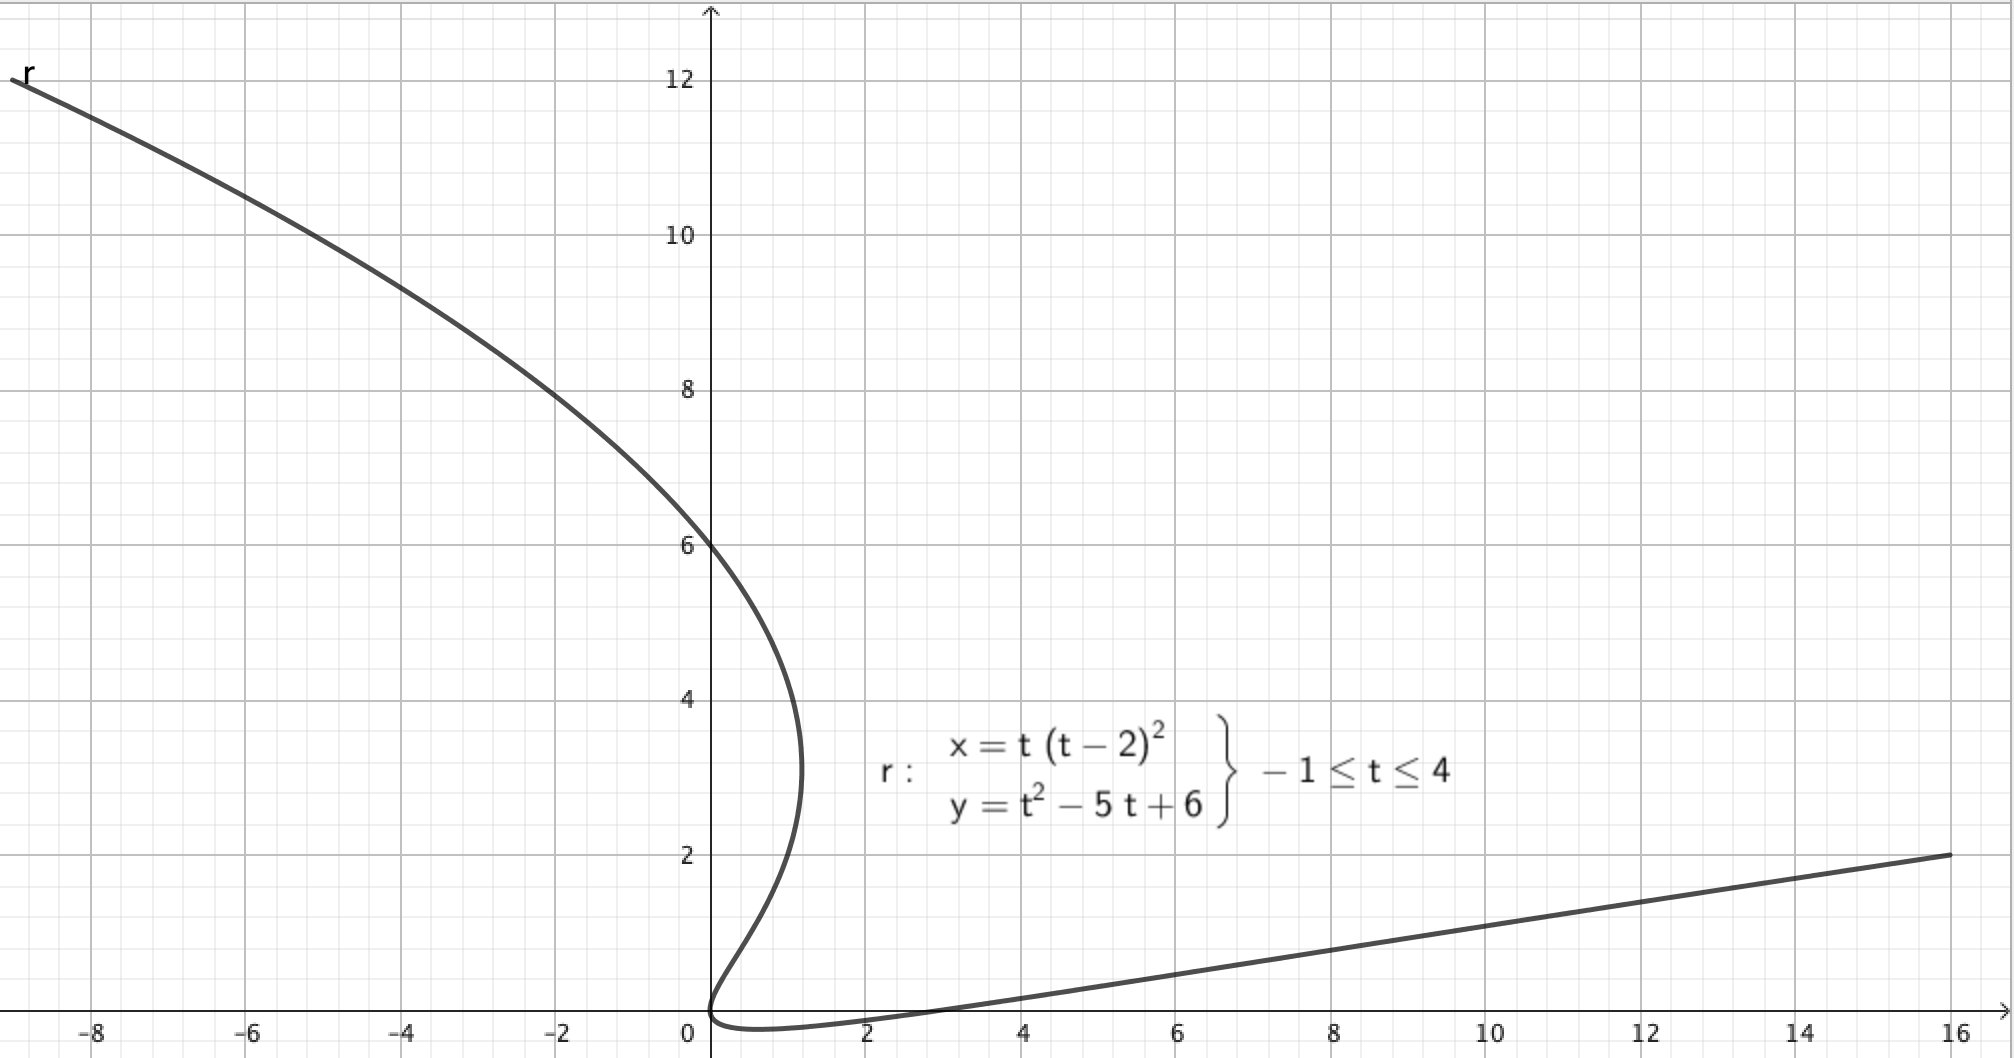
\includegraphics[width=\textwidth]{vektorfunktion.png}
\end{center}
  \caption{Banekurven for $\va{r}(t)$ tegnet i GeoGebra}
\label{fig:vektorfunktion}
\end{figure}
\begin{question}{}{}
  En vektorfunktion $\va{r}:[-10;10]\to \mathbb{R}$ er givet ved 
  \[
  \va{r}(t)=\mqty(2t^3-3t^2-36t\\ t^2) 
  \] 
  Det oplyses, at der findes præcis ét dobbeltpunkt på banekurven for $\va{r}(t)$
  \begin{itemize}
    \item[a.] Bestem dobbeltpunktets koordinater ved beregning.
  \end{itemize}
\end{question}
\sol \\
\textbf{a.} Ved dobbeltpunktet er $t$-værdien forskellig, men positionsvektoren er den samme.
Vi kalder de to $t$-værdier ved dobbeltpunktet for $t$ og $x$. 
Vi skal altså løse ligningssystemet, hvor $x\neq t$:
\begin{equation*}
\begin{split}
  2t^3-3t^2-36t&=2x^3-3x^2-36x \\
  t^2&=x^2
\end{split}
\end{equation*}
Da vi ikke vil have $x=t$, så har vi
\[
t^2=x^2 \land x\neq t \implies t=-x
\] 
Vi laver en substitution.
\begin{equation*}
\begin{split}
  -2x^3-3x^2+36 x=2x^3-3x^2-36x &\iff 4x^3-2 \cdot 36x=0\\ 
  &\iff x \cdot (x^2-18)=0 \\ 
  &\implies x=0 \lor x^2=18\\ 
  &\iff x=0 \lor x=3 \sqrt{2} \lor x=-3 \sqrt{2}
\end{split}
\end{equation*}
$x$ kan dog ikke være lig med 0, da det modstrider vores antagelse om, at $x\neq t$.
Altså har vi løsningerne
\begin{equation*}
\begin{split}
  x=3 \sqrt{2} &\land t=-3 \sqrt{2} \\ 
  x=-3 \sqrt{2} &\land t=3 \sqrt{2} 
\end{split}
\end{equation*}
Vi finder positionsvektoren til dobbeltpunktet ved at tage vektorfunktionen af en af de fundne $t$-værdier.
\begin{equation*}
\begin{split}
  \va{r}(t)&=\mqty(2 \cdot \left(3 \sqrt{2} \right)^3-3 \cdot \left(3 \sqrt{2} \right)^2 - 36 \cdot 3 \sqrt{2} \\ \left(3 \sqrt{2} \right)^2) \\
  &=\mqty(-54\\ 18) 
\end{split}
\end{equation*}
Altså må dobbeltpunktets koordinater være $(-54, 18)$.
\end{document}
